\chapter{Методика разработки, исследования динамики и испытаний систем управления бортовыми оптико-электронными приборами с применением информационных технологий} \label{ch:ch2}

\begin{comment}
В настоящее время наиболее распространены в народном хозяйстве и военной технике комплексированные оптико - электронные системы (КОЭП) визуализации, включающие в себя каналы наблюдения и зондирования в широком спектре волн оптического диапазона \cite[]{Tarasov},\cite[]{Belyakov},\cite[]{Karpov},\cite[]{Torshina}. Появление на рынке матричных фотоприемников расширило возможности КОЭП и К(комплексов). Несмотря на интенсивное развитие теории и методов расчета и совершенствование бортовых автоматических КОЭП и К возникают ряд вопросов, влияющих на качество получаемой оптической информации, в частности – это вопросы динамики и качества управления и увязки их с оптическими характеристиками каналов визуализации \cite[]{Belyakov},\cite[]{Karpov}, \cite[]{Baloev16}, \cite[]{Karpov17}.
\end{comment}

%Рассматриваются алгоритмы методики
Вопросами моделирования, исследования динамики, разработки и испытаний систем управления бортовыми оптико-электронными приборами для решения задач наблюдения в разных постановках и допущениях посвящены работы \cite{Tarasov,Belyakov,Torshina,Ivanov18,Bessekerski20,Karpov,BLDC_Stefan,Baloev16,Karpov17,Gerasin19,Molin21,Sokolski22,Karpov23,Babaev38-a2-13,Bessekerski-a2-14,Malivanov-a2-9,Babatko-a2-17}. 
Ниже в развитие работы \cite[]{Tarasov} рассматривается методика разработки и исследования систем автоматического управления (\hyperref[acroSAU]{САУ}) \hyperref[acroEOS]{ОЭП} с использованием замкнутых процедур исследования от разработки математических моделей до испытаний на борту носителя.
%\cite[]{Tarasov}-\cite[]{BLDC_Stefan}.

%Оптико-электронные приборы (\hyperref[acroEOS]{ОЭП}) авиационного, морского, наземного и космического базирования нашли широкое применение при выполнении задач наблюдения и охраны, в том числе при решении народнохозяйственных задач и задач обороны и безопасности.

% Появление на рынке матричных фотоприемников расширило возможности \hyperref[acroEOS]{ОЭП} и комплексов. Несмотря на интенсивное развитие теории и методов расчета и совершенствование бортовых автоматических \hyperref[acroEOS]{ОЭП} возникает ряд вопросов, влияющих на качество получаемой оптической информации, в частности – это вопросы динамики и качества управления и увязки их с характеристиками каналов визуализации \cite[]{Tarasov},\cite[]{Belyakov}, \cite[]{Baloev16}, \cite[]{Karpov17}, \cite[]{Gerasin19}. 

 


\section{Методика разработки, исследования и испытания динамики \hyperref[acroSAU]{САУ}} \label{sec:ch2/sec1-}

В настоящее время широко рекламируются и применяются комплексированные бортовые \hyperref[acroEOS]{ОЭП} визуализации, включающие в себя каналы наблюдения и зондирования в широком спектре волн оптического диапазона, для применения в народном хозяйстве и военной технике \cite{Tarasov,Belyakov,Torshina,Ivanov18}.

Наличие нелинейных перекрестных связей, нестационарности параметров в ОУ и нестационарностей в регуляторе, затрудняет применение известных методов в теории управления. В связи с этим ниже рассматривается интерактивная процедура  исследования САУ.

Разработка \hyperref[acroSAU]{САУ} \hyperref[acroEOS]{ОЭП} модернизируемых или вновь создаваемых начинается с выбора приемлемого варианта. Для этого решается много критерийная задача оптимизации с учетом ряда противоречивых технико-экономических (Т-Э) требований: 
надежность - $\alpha_{1}$, 
масса объекта управления (ОУ) - $\alpha_{2}$, 
потребляемая энергия - $\alpha_{3}$, 
конкурентоспособность - $\alpha_{4}$, 
стоимость - $\alpha_{5}$, 
погрешность \hyperref[acroSAU]{САУ} - $\alpha_{6}$, 
полоса пропускания \hyperref[acroSAU]{САУ} - $\alpha_{7}$; 
качество изображения - $\alpha_{8}$, 
время наведения - $\alpha_{9}$ , 
характеристики объектива -$\alpha_{10}$, 
характеристики приемника излучения - $\alpha_{11}$, которые определяются из технического задания (ТЗ) на \hyperref[acroEOS]{ОЭП} методом экспертных оценок специалистов в этих областях науки и техники с учетом предварительных расчетов и исследований. Критерий выбора приемлемого (\textit{i}) варианта определяется по формуле []:

\begin{equation}
\label{eq:p2:1}
\begin{alignedat}{2}
k_i=min\sum_{j=1}^n{\gamma _{ji}\alpha _{ji}}; \gamma _{j}=j ; i=m
\end{alignedat}
\end{equation}
где \textit{m} – число вариантов, \textit{n} – число Т-Э параметров, $\gamma_{ij}$ – весовые коэффициенты, $\alpha_{ji}$ – Т-Э параметры. Для выбранных приемлемых вариантов \hyperref[acroSAU]{САУ} (не более двух) в соответствии с методикой, изложенной ниже проводится исследование их динамики. За критерий качества \hyperref[acroSAU]{САУ} принимаем совокупность динамических характеристик каналов управления, удовлетворяющих условиям:

\begin{equation}
\label{eq:p2:2}
\begin{alignedat}{2}
\varDelta \alpha _k\leqslant \varDelta \alpha _{k}^{\textit{доп}},
\\
\,\,\,\,\varDelta \dot{\alpha}_k\leqslant \varDelta \dot{\alpha}_{k}^{\textit{доп}},
\\
\tau < \tau^\textit{доп},
\\
\,\,\,\,\,\,M_k\leqslant \text{1.05..1.25,}
\\
\,\,\,\,\left| \left. \varDelta \varphi_k \right| \right. \geqslant \left( 45-60 \right) ^0,
\\
\,\,\,\,\left| \left. \varDelta L_k \right|\geqslant \,\,\textit{6 дб}, \right. 
\end{alignedat}
\end{equation}
где $\varDelta \alpha^{\textit{доп}}_{k}$, 
$\varDelta \dot{\alpha}^{\textit{доп}}_{k}$, 
$\varDelta \alpha _k$, 
$\varDelta \dot{\alpha}_k$ 
- допустимые и установившиеся значения динамических погрешностей \hyperref[acroSAU]{САУ} по углу и угловой скорости при действии возмущений, полученных в условиях, близких к реальной эксплуатации \hyperref[acroSAU]{САУ}, \textit{k= 1,2,...} - номер канала управления, $\tau, \tau^\textit{доп}$ - допустимое и установившееся время наведения, $М_k$ – показатель колебательности, $\varDelta \varphi_k$, $\varDelta L_k$ –запасы устойчивости по фазе и по амплитуде, полученные из логарифмической частотной характеристики (ЧХ) разомкнутой системы.% \cite[]{Bessekerski20}.

Согласно разработанной методике алгоритм разработки \hyperref[acroSAU]{САУ} и исследования их динамики представлен в виде 7-и последовательных интерактивных процедур с использованием 29-ми блоков разработки и исследования (рисунок~\ref{fig:tikz_example}):
\newcounter{iter}

\stepcounter{iter} \arabic{iter}. Выполняется последовательная процедура оценки функции передачи модуляции (ФПМ) бортовой излучающей оптико-электронной системы (БИзОЭП) (разработки расчетной и математической моделей, декомпозиции) с применением компьютерных технологий (Solid Works, MathCAD, MATLAB): (рисунок~\ref{fig:tikz_example}: 1-5,27,28).
	
\stepcounter{iter} \arabic{iter}. Далее выполняется процедура идентификации параметров математической модели до выполнения критериев качества (\ref{eq:p2:2}) с доопределением параметров, моделей и структуры при необходимости (рисунок~\ref{fig:tikz_example}: 1-5,27,28).
	
\stepcounter{iter} \arabic{iter}. проводится интерактивный синтез алгоритмов управления изолированных каналов \hyperref[acroSAU]{САУ} частотным методом \cite[]{Bessekerski20} (рисунок~\ref{fig:tikz_example}: 8,9,25,28) до выполнения критериев качества (\ref{eq:p2:2}). 
	
\stepcounter{iter} \arabic{iter}. На основании полученной информации проводится разработка и изготовление масштабного динамического макета \hyperref[acroEOS]{ОЭП} (ОУ, приводов, встроенных датчиков с обеспечением адекватности их динамическим характеристикам) с применением 3D - принтера (рисунок~\ref{fig:tikz_example}: 10). Далее проводится исследование динамики пространственного движения макета \hyperref[acroSAU]{САУ} с использованием синтезированных алгоритмов управления (рисунок~\ref{fig:tikz_example}: 11-12). Если требования критериев качества (\ref{eq:p2:2}) не выполняются, то проводятся последовательно циклы итерационных исследований динамики \hyperref[acroSAU]{САУ}: (рисунок~\ref{fig:tikz_example}: 24,25,28) до обеспечения критериев качества (\ref{eq:p2:2}), заключающихся в выборе параметров регулятора и ОУ макета.
	
\stepcounter{iter} \arabic{iter}. Далее переходим к исследованию нелинейной пространственной КИМ с применением MATLAB: (рисунок~\ref{fig:tikz_example}: 13-15). Если критерии (\ref{eq:p2:2}) не выполняются, то переходим к 23,25 или 28, где доопределяем число степеней свободы математической модели и её параметры, параметры регулятора \hyperref[acroSAU]{САУ} путем последовательных предыдущих итераций исследований до выполнения критериев (\ref{eq:p2:2}). C учетом полученной информации доопределяем: необходимые конструктивные доработки ОУ, \hyperref[acroSAU]{САУ}; приемлемые варианты построения \hyperref[acroSAU]{САУ}, а также в случае необходимости уточняем критерии (\ref{eq:p2:2}) и задачи, которые может решать \hyperref[acroSAU]{САУ}, а также ограничения и нелинейности в контурах управления. По результатам исследования делается заключение о необходимости изготовления опытного образца \hyperref[acroSAU]{САУ} или проведения дальнейших исследований.
	
\stepcounter{iter} \arabic{iter}. После выполнения критериев (\ref{eq:p2:2}) переходим к испытаниям опытного образца \hyperref[acroSAU]{САУ} в режимах наведения и стабилизации на стендах в соответствии с методиками испытаний и требований ТЗ: (рисунок~\ref{fig:tikz_example}: 16-17). Если критерии (\ref{eq:p2:2}) не выполняются, то переходим на 6-ю последовательность процедур: (рисунок~\ref{fig:tikz_example}: 17,22,28), (рисунок~\ref{fig:tikz_example}: 17,22,25), которые при необходимости включает в себя три предыдущих. Результаты исследований фиксируют в протоколе испытаний и делают заключение о необходимости доработок \hyperref[acroSAU]{САУ} или допуске их к испытаниям на борту. 
	
\stepcounter{iter} \arabic{iter}. В заключении переходим к испытаниям \hyperref[acroSAU]{САУ} на борту в соответствии с методиками натурных испытаний и требований ТЗ: (рисунок~\ref{fig:tikz_example}: 18-19). Если критерии (\ref{eq:p2:2}) не выполняются, то переходим на 7-ую последовательность процедур: (рисунок~\ref{fig:tikz_example}: 21,29). Результаты испытаний и требования к техническим характеристикам \hyperref[acroSAU]{САУ} фиксируем в протоколе испытаний и делаем заключение о необходимости доработок \hyperref[acroSAU]{САУ} или допуске их к дальнейшему производству.

Была апробирована при разработке ряда \hyperref[acroSAU]{САУ} \hyperref[acroEOS]{ОЭП} \cite{Belyakov,Karpov,Baloev16,Karpov17,Gerasin19,Molin21}. Каждому из блоков приведенных на рисунке~\ref{fig:tikz_example} присущи своя специфика и его математическое или логическое описание.

\begin{figure}[ht]
	\centering
	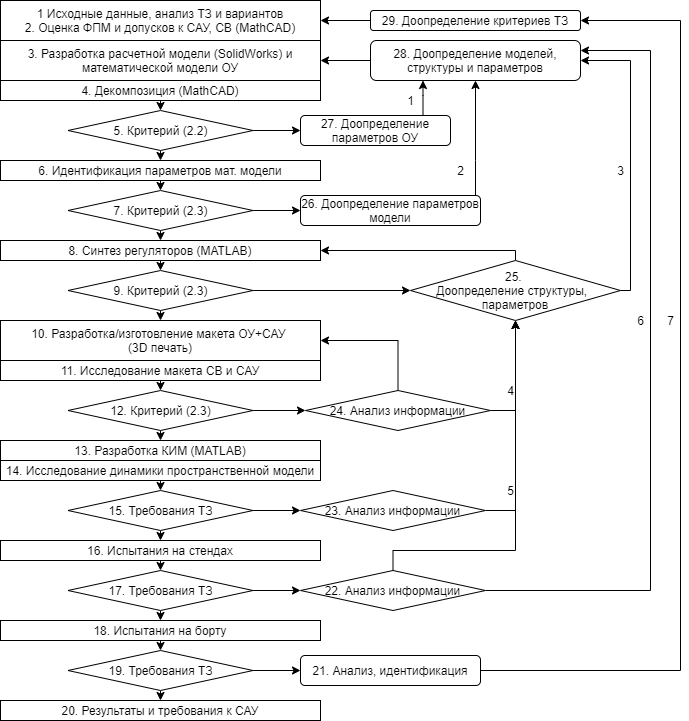
\includegraphics[width=0.9\linewidth]{algoritm} 
	\caption{Блок-схема алгоритма методики разработки и исследования динамики САУ}
	\label{fig:tikz_example}
\end{figure}

\newpage

\section{Оценка допуска на точность стабилизации изображения} \label{sec:ch2/sec2}
Определение допустимых динамических погрешностей визуализации объекта наблюдения (ОН) является ключевым вопросом в разработке бортовых ОЭП. В указанных работах \cite{Molin21,Sokolski22,Belyakov} рассматриваются  уточненные формулы  (требования) позволяющие оценить допустимые динамические погрешности  стабилизации оси визирования излучающих ОЭП в режимах наведения и слежения за ОН.

Для изучения процесса формирования изображения с учетом множества факторов, влияющих на формирование, преобразование и передачу качества изображения, рассмотрим функциональную схему одного из вариантов объединенного ОЭП и СОЭП (рисунок~\ref{fig:oep_sch}), представляющего собой совокупность тепловизионной системы \hyperref[acroTVS]{(ТВС)}, телевизионной системы \hyperref[acroTS]{(ТС)}, лазерного дальномера (ЛД), а так же системы постановки помех. В результате действия внешних возмущений, возмущений, идущих от носителя, и наличия управления \hyperref[acroEOS]{ОЭП} в пространстве остается не компенсированный сдвиг изображения (динамическая погрешность).

\begin{figure}[ht]
	\centering
	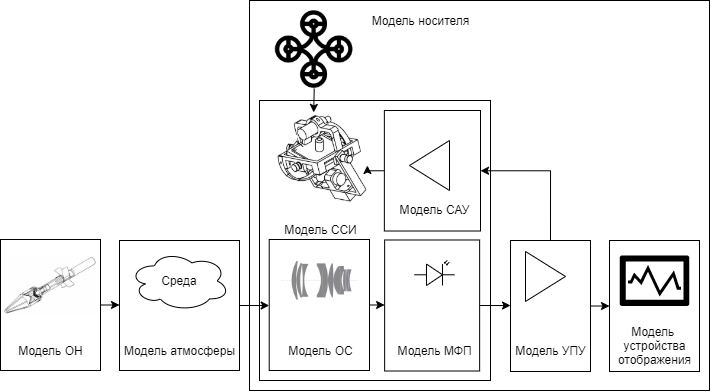
\includegraphics[width=0.8\linewidth]{FPM_scheme} 
	\caption{Функциональная схема обобщённой модели \hyperref[acroEOS]{ОЭП}}
	\label{fig:oep_sch}
\end{figure}

Это приводит к изменению структуры изображения аналогично влиянию аберраций, т.е. к ухудшению качества изображения, зависящего от величины и характера изменения динамических погрешностей управляющих систем. Для оценки допуска на точность стабилизации изображения используют частотный критерий качества изображения \hyperref[acroEOS]{ОЭП} – функцию передачи модуляции (\hyperref[acroFPM]{ФПМ}) \cite[]{Tarasov}.

Оценка качества изображения управляемых \hyperref[acroEOS]{ОЭП} определяется на основе анализа произведения \hyperref[acroFPM]{ФПМ} элементов оптико-электронного тракта, формирующих изображение и влияющих на качество изображения. В рамках принятой структуре \hyperref[acroEOS]{ОЭП} его \hyperref[acroFPM]{ФПМ} должна удовлетворять условию \cite[]{Ivanov18,Molin21}.

\begin{equation}
\label{eq:p2:2.5}
\begin{alignedat}{2}
T_{\textit{ОЭП}}( \nu )=
T_{\textit{ат}}(\nu)T_{\textit{об}}(\nu)T_{\textit{фп}}(\nu)T_{\textit{упу}}(\nu)T_{\textit{м}}(\nu)
T_{\textit{САУ}}(\nu)>T_{\textit{ОЭC}}^{\textit{доп}}(\nu)
\end{alignedat}
\end{equation}
где 
$T_{\textit{оэп}}(\nu)$ – \hyperref[acroFPM]{ФПМ} \hyperref[acroEOS]{ОЭП}, 
$\nu$ – пространственная частота, 
$T_{\textit{ОЭП}}^{\textit{доп}}(\nu)$ – допустимая \hyperref[acroFPM]{ФПМ} \hyperref[acroEOS]{ОЭП}, 
$T_\textit{ат}(\nu)$ – \hyperref[acroFPM]{ФПМ} атмосферы, 
$T_\textit{oб}(\nu)$ – \hyperref[acroFPM]{ФПМ} объектива, 
$T_\textit{фп}(\nu)$ – \hyperref[acroFPM]{ФПМ} фотоприемника, 
$T_\textit{упу}(\nu)$ – \hyperref[acroFPM]{ФПМ} преобразования оптической информации, вид которых можно найти в \cite[]{Tarasov},
$T_\textit{фп}(\nu)$ – \hyperref[acroFPM]{ФПМ} устройства вывода (монитор), 
$T_{\textit{САУ}}(\nu)$ – \hyperref[acroFPM]{ФПМ} сдвига изображения (динамической погрешности \hyperref[acroSAU]{САУ}), зависящая от вида динамического смещения изображения: линейного (Л) - $\dot{x}(t) = Vt$, 
гармонического (Г) - $x(t)=a_{0}\sin{\omega t}$ и 
случайного (СЛ) \cite{Tarasov,Sokolski22}.

Приведем формулы ФПМ для подсистем, которые используются в предлагаемой математической модели ОЭС для одномерного случая.
\newcounter{FPMc}

\stepcounter{FPMc} \arabic{FPMc}. ФПМ атмосферы  учитывает ФПМ рассеяния   и ФПМ турбулентности  

\stepcounter{FPMc} \arabic{FPMc}. ФПМ модели ОС для бортовых ОЭП по каждому каналу наблюдения может быть представлена  в виде трех составляющих [4] (дифракционной, аберрационной и расфокусировки):

\stepcounter{FPMc} \arabic{FPMc}.Для современных ОЭП характерным является использование модели матричного фотоприёмника. Его ФПМ определяется как размерами элемента, так и недостаточно высокой эффективностью переноса заряда между соседними ячейками системы считывания, а также электрическими перекрестными связями между ними, вызывающими диффузионное расплывание заряда, что имеет место для ПЗС-структур [4, 5]

\stepcounter{FPMc} \arabic{FPMc}.ФПМ УПУ описывают амплитудно-частотной характеристикой однозвенного интегрирующего фильтра [4]

\stepcounter{FPMc} \arabic{FPMc}.ФПМ  систем отображения (монитора) принимают в виде [4]

\stepcounter{FPMc} \arabic{FPMc}.ФПМ ССИ, обеспечивающих качество изображения, представлена в виде ФПМ: ССк, ССл, САФ, СВ. Перечисленные ФПМ зависят от величин угловой скорости движения изображения, расфокусировки (t) и вибраций. 
В зависимости от вида движения изображения ФПМ ССк, ССл, СВ, которые представляют следующими выражениями [6, 7]: 


\begin{equation}
\label{eq:p2:3}
\begin{alignedat}{2}
T_{\textit{ОЭC}}^{\textit{доп}}\left(\nu{}\right)=
\frac{N{\gamma{}}_\textit{и}}{2\sin{\left(N\frac{{\gamma{}}_\textit{и}}{2}\right)}}
\exp{\left[-\frac{{\left(N{\gamma{}}_p\right)}^2}{16\ln{\left(2m\right)}}\right]}
\end{alignedat}
\end{equation}

\begin{equation}
\label{eq:p2:4}
\begin{alignedat}{2}
T_{\Sigma{}}^{\textit{доп}}\left(\nu\right)=\exp{\left(-2{\pi{}}^2{\sigma{}}^2\nu^2\right)}
\end{alignedat}
\end{equation}
где 
$\nu$ – пространственная частота, 
$m$ - отношение сигнал/шум, 
$\gamma_\textit{и}$ - угловой размер источника излучения, 
$\gamma_\textit{p}$ - угловое разрешение \hyperref[acroEOS]{ОЭП}. 

Тогда в частном случае допустимая \hyperref[acroFPM]{ФПМ} \hyperref[acroSAU]{САУ} (системы слежения (Л, Г), системы виброзащиты (СВ), автоматической фокусировки (САФ)) определится соответственно: 

\begin{equation}
\label{eq:p2:6}
\begin{alignedat}{2}
T_{\textit{САУ}}\left(\nu\right)=
T_\textit{Л}\left(\nu\right)T_\textit{Г}\left(\nu\right)T_{\textit{СВ}}\left(\nu\right)T_{\textit{САФ}}\left(\nu\right)\geq{}T_{\textit{САУ}}^{\textit{доп}}(\nu)= \\
\dfrac{ T_{\textit{оэп}}^{\textit{доп}}(\nu) }{ T_{\textit{ат}}(\nu)T_{\textit{об}}(\nu)T_{\textit{фп}}(\nu)T_{\textit{пои}}(\nu) }
\end{alignedat}
\end{equation}

\begin{equation}
\label{eq:p2:7}
\begin{alignedat}{3}
T_\textit{Л}\left(N\right)=Sinc(\pi{}VtN) , \\
T_{\textit{Г}}(\nu)=J_0\left(2\pi{}a_0N\right) , \\
T_{\textit{СВ}}\left(N\right) = exp[-2{(\pi{}a_{\textit{ср}}N)}^2]
\end{alignedat}
\end{equation}

где $T_{\textit{САФ}}(\nu)$ – ФПМ САФ; 
$V$ – допустимая скорость движения изображения; 
$J_0(\dot)$ - функция Бесселя нулевого порядка, 
$a_0$ –допустимая амплитуда гармонических колебаний, 
$a_{\textit{ср}}$ – среднее значение допустимой амплитуды случайного сдвига изображения. 
Выражения для оценки допустимых динамических погрешностей для САУ и СВ можно найти в \cite[]{Karpov}, \cite[]{Karpov23}. Допуск на точность САФ для фотообъективов в видимой области спектра, инфракрасных систем можно найти в \cite[]{Tarasov}, \cite[]{Belyakov}.

Пространственная расчетная частота $\nu_p$ должна соответствовать средним пространственным частотам (частоте Найквиста ($N_{\textit{н}} (\textit{мм}^{-1})$ либо $f_H (\textit{рад}^{-1})$), которая выбирается c учетом условий \cite[]{Tarasov}: 

\begin{equation}
\label{eq:p2:8}
\begin{alignedat}{2}
N_H=0.5 N_{\textit{выб}}\leq{}N_{\textit{гр}},
N_{\textit{гр}}=\frac{D}{1.22\lambda{}f^{'}},\\
f_H=\frac{X_\textit{э}}{2f^{'}},
f_{\textit{гр}}=\frac{D}{\lambda{}}(\textit{рад}^{-1}),
f_{\textit{выб}}=\frac{n_{\textit{э}}}{2\omega{}},\\
D\geq{}\frac{1.22 k_{\textit{аб}}\lambda{}}{h_{\textit{кр}}},
N_x=\frac{N_{\textit{д}}l}{h_{\textit{кр}}f^{'}},\\
f_x=\frac{N_{\textit{д}}l}{h_{\textit{кр}}},
f_{xy}=\frac{N_{\textit{д}}l}{\sqrt{h_{\textit{крx}}h_{\textit{крy}}}}=\sqrt{f_x^2+f_y^2},\\
\Delta{}{\omega{}}_p=\frac{2h_{\textit{кр}}}{N_{\textit{д}}l},
\Delta{}{\omega{}}_{\textit{аб}} =\frac{2.44 k_{\textit{аб}}\lambda{}}{D},
\Delta{}{\omega{}}_{\textit{э}} =\frac{d_{\textit{э}}}{f^{'}},\\
\frac{D}{f^{'}}=\frac{2.44 k_{\textit{аб}}\lambda{}}{d_{\textit{э}}},\\
\end{alignedat}
\end{equation}

где 
$N_{\textit{гр}}$ – граничная пространственная частота, 
$f_{\textit{выб}}$ – частота выборки, 
$X_{\textit{э}} ,n_{\textit{э}}$ –период расположения и число элементов фотоприемника, 
$2\omega$ - поле зрения ОЭП, 
$k_{\textit{аб}}$ – коэффициент, учитывающий аберрации объектива, 
$h_{\textit{кр}}$ – критический размер объекта наблюдения (ОН), 
$l$ – расстояние до ОН, 
$N_{x} , f_{x}$ – пространственные частоты, соответствующие критериям Джонсона, 
$N_{\textit{д}}$ – числа элементов разрешения (критерии Джонсона – обнаружения, классификации, распознавания и идентификации), 
$f_{xy}$ - пространственная частота Джонсона в двух ортогональных направлениях \textit{x} и \textit{y}, 
$\Delta{}{\omega{}}_p$ – требуемое геометрическое угловое разрешение, необходимое для наблюдения, 
$\Delta{}{\omega{}}_{\textit{аб}}$ – минимальное угловое значение кружка рассеяния объектива с учетом аберраций, 
$\Delta{}{\omega{}}_{\textit{э}} , d_{\textit{э}}$ – угловой и линейный размеры элемента чувствительного слоя приемника излучения. 

Если при $N \ge N_p$ качество изображения ОЭС будет удовлетворять условию $Т(\nu) \ge 0.8$, то оно считается хорошим. Таким образом, используя (\labelcref{eq:p2:6,eq:p2:7,eq:p2:8}), можно определить допустимые динамические погрешности, обеспечивающие выполнение условия (\ref{eq:p2:6}).

Методика оценки допусков:

1.

2.


\section{Разработка математической модели} \label{sec:ch2/sec3}

При разработке ОЭП одной из важнейших задач является управление направлением линии визирования в пространстве. Оно осуществляется, как правило, двумя способами: путем управления всем устройством информационных каналов (ОЭП 1-го типа) и управлением положением отдельных оптических элементов (зеркал, призм) (ОЭП 2-го типа) \cite[]{Karpov23}. Оба способа построения управляющих ОЭП имеют свои особенности и широко применяются.

Для построения математических моделей относительного движения ОЭП (движения относительно корпуса летательного аппарата (ЛА), на котором они устанавливаются) используются уравнения Лагранжа II-го рода. За инерциальную систему отсчета принимается система координат, связанная с поверхностью Земли. Для записи уравнений Лагранжа II-го рода используется смешанный метод Жильбера \cite[]{Belyakov}, \cite[]{Baloev16}. Для изучения динамики ОЭП 1-го типа моделируется двумя абсолютно твердыми телами: «вилка» - азимутальный блок, в которой установлено второе тело - оптико-электронный блок (ОЭБ). Оси вращения «вилки» и ОЭБ взаимно перпендикулярны и пересекаются. Угол поворота «вилки» по азимуту – $\alpha$, угол поворота ОЭБ по углу места –$\beta$. Математическая модель относительного движения ОЭП 1-го типа определяется следующим матричным уравнением \cite[]{Karpov23}:

\begin{equation}
\label{eq:p2:6-}
\begin{alignedat}{2}
A_c\left(q_c\right){\ddot{q}}_c+B_c\left(t,q_c\right){\dot{q}}_c+Q_c\left(t,q_c\right)+\\
F_c\left(t,q_c\right)+F1_c\left(q_c,{\dot{q}}_c\right)=\frac{c_M}{r}u-M_{\textit{тр}}
\end{alignedat}
\end{equation}

где
$q_c=\left(\begin{array}{cc}
\alpha{} \\
\beta{}
\end{array}\right)$, 
$u=\left(\begin{array}{
	cc}
u_1 \\
u_2
\end{array}\right)$

$M_{\textit{тр}}=\left(\begin{array}{
		cc}
	M_{\textit{тр.1}}sign\left(\dot{\alpha{}}\right) \\
	M_{\textit{тр.2}}sign\left(\dot{\beta{}}\right)
\end{array}\right)$, 
$A_c\left(q_c\right),B_c\left(t,q_c\right)$ – матрицы-функции размерности $2 \times 2$,
$Q_c\left(t,q_c\right),F_c\left(t,q_c\right),F1_c\left(q_c,{\dot{q}}_c\right)$ – столбцы-функции размерности $2 \times 1$,
$u_1$, $u_2$ - управляющее сигналы на моментных двигателях по азимуту и углу места. 

Азимутальный блок и угломестный блок ОЭП 2-го типа совместно с соосными приводами моделируется двумя подвижными твердыми телами, установленными в кардановом подвесе прибора, который закреплен на ЛА. Положение этих тел относительно корпуса однозначно определяется углами поворотов азимутального ($\phi_1$) и угломестного ($\phi_2$) блоков. Математическая модель относительного движения ОЭП 2-го типа определяется следующим матричным уравнением \cite[]{Baloev16}:

\begin{equation}
\label{eq:p2:7-}
\begin{alignedat}{2}
A\left(\phi{}\right)\ddot{\phi{}}+N\left(\phi{},\dot{\phi{}}\right)+H\left(\phi{},{\omega{}}_1\right)\dot{\phi{}}+\\
L\left(\phi{}\right){\epsilon{}}_1(t)-\Omega{}\left(\phi{},{\omega{}}_1\right)=\frac{c_M}{r}u-M_{mp}-P\left(\phi{},a\right)
\end{alignedat}
\end{equation}

$\phi{}=\left(\begin{array}{
	cc}
{\phi{}}_1 \\
{\phi{}}_2
\end{array}\right)$, $u=\left(\begin{array}{
	cc}
u_1 \\
u_2
\end{array}\right),$ $M_{mp}=\left(\begin{array}{
	cc}
M_{\textit{mp.1}} \dot{\phi_1} \\
M_{\textit{mp.2}} \dot{\phi_2}
\end{array}\right)$,

$A\left(\phi{}\right),H\left(\phi{},{\omega{}}_1\right)$ – матрицы-функции размерности $2 \times 2$, $L(\phi)$– матрица-функция размерности $2 \times 3$,
$P\left(\phi{},a\right),N\left(\phi{},\dot{\phi{}}\right),\Omega{}\left(\phi{},{\omega{}}_1\right)$ –столбцы-функции размерности $2 \times 1$,
${\omega{}}_1(t)=\left(\begin{array}{
	ccc}
{\omega{}}_{X1}(t) \\
{\omega{}}_{Y1}(t) \\
{\omega{}}_{Z1}(t)
\end{array}\right)$
, ${\epsilon{}}_1(t)=\left(\begin{array}{
	ccc}
{\dot{\omega{}}}_{X1}(t) \\
{\dot{\omega{}}}_{Y1}(t) \\
{\dot{\omega{}}}_{Z1}(t)
\end{array}\right)=\left(\begin{array}{
	ccc}
{\epsilon{}}_{X1}(t) \\
{\epsilon{}}_{Y1}(t) \\
{\epsilon{}}_{Z1}(t)
\end{array}\right)$
– векторы, составленные из проекций векторов угловой скорости и углового ускорения ЛА на оси, связанные с корпусом ОЭП. Значения элементов матриц-функций определяется величинами осевых и центробежных моментов инерции, положением центров масс и массами тел прибора. В уравнениях (\labelcref{eq:p2:6-,eq:p2:7-,}) зависимость от времени определяется уравнениями движения ЛА ($\omega_1(t)$).

\section{Идентификация параметров} \label{sec:ch2/sec4}

Одним из наиболее эффективных методов построения математических моделей является экспериментальный метод – верификация (идентификация). Суть идентификации состоит в том, что по реакции $x(t)$ исследуемой САУ (или её части) на известные виды воздействий $у(t)$ определяют динамические характеристики САУ (или ее части), а по ним и ее математическую модель. Процедура идентификации по переходным и частотным характеристикам САУ с заданным критерием адекватности реальной системе включает в себя интерактивный процесс построения расчетных и математических моделей САУ \cite[]{Karpov}. Пусть:

\begin{enumerate}
	\item Модель САУ управляема и наблюдаема \cite[]{Bessekerski20} и описывается системой 
	\begin{equation}
	\label{eq:p2:8-}
	\begin{alignedat}{2}
	\alpha{}={\left(E+W(P)\right)}^{-1}W(p)y
	\end{alignedat}
	\end{equation}
	где $W_{ij}(р)={\left\Vert{}W_{ij}(р)\right\Vert{}}_{rxr}$	
	передаточная матрица разомкнутой системы, 
	$E$ – единичная матрица,
	$\alpha$ - вектор регулируемых координат, 
	$у$ - вектор управления, 
	$r$ – число регулируемых координат. 
	Обозначим переходные процессы исходной модели ($М_I$) и последующих моделей ($M_k$, k=2,3...), 
	определяемых далее в процессе идентификации, при известных $\alpha_k (t_0 ), у_k (t)$ через 
	$\alpha_{i} (t)={\left\Vert{} \alpha_{i}(v^k,t) \right\Vert{}}_{rx1}$, 
	а частотные характеристики (ЧХ) разомкнутых САУ через 
	$W_{ij}(j\omega) = {\left\Vert{} W^k_{ij}(v^k, j\omega) \right\Vert{}}_{rxr}$. 
	Здесь и далее: $k$ – номер модели, $v^k$ – вектор варьируемых параметров k–ой модели, $D_{v^k}$ - область существования параметров
	\begin{equation}
	\label{eq:p2:9-}
	\begin{alignedat}{2}
	v^k \in D_{v^k} (k= 1,2,...)
	\end{alignedat}
	\end{equation}	
	\item Получены ЧХ элементов матрицы 
	$\tilde{W}_{ij}(j\omega) = {\left\Vert{} \tilde{W}_{ij}( j\omega) \right\Vert{}}_{rxr}$
	реальной САУ в рабочем диапазоне частот 
	$\Omega{}=\left[{\omega{}}_1,{\omega{}}_2\right]$ 
	разомкнутых каналов управления и переходные процессы 
	$\tilde{\alpha}_{i}(t) = {\left\Vert{} \tilde{\alpha}_{i}(i) \right\Vert{}}_{rx1}$
	в процессе нормальной эксплуатации при заданных 
	$\alpha(t_0)$, $y(t)$ за время $T=[t_0,t_1]$.
	
	Оценка степени адекватности модели и идентичности каждой полученной модели реальной системе, а также уточнение моделей может оцениваться следующими критериями адекватности: 
	
	\begin{equation}
	\label{eq:p2:10-}
	\left. %ВАЖНО: точка после слова left делает скобку неотображаемой
	\begin{aligned}
	\min_v \max_\omega \left| L_m\left| \tilde{W}_{ij}(j\omega) \right| - L_m\left| {W}^k_{ij}(v^k, j\omega) \right| \right| &\leq \varDelta L(\omega) \\
	\min_v \max_\omega \left| arg \tilde{W}_{ij}(j\omega) - arg {W}^k_{ij}(v^k, j\omega) \right| &\leq \varDelta \phi(\omega) \\
	\dfrac{1}{T}\int^T_0\left| \alpha_i(t,v^k)- \tilde{\alpha}_i(t) \right| dt &\leq \epsilon_i
	\end{aligned}\right\}
	\end{equation}
	где $Lm(x)=20lg(x)$, $\varDelta L(\omega)$, $\varDelta \phi(\omega)$, $\epsilon_i$ – невязки, характеризующие погрешность идентификации. Невязки $\varDelta L(\omega)$, $\varDelta \phi(\omega)$, $\epsilon_i$ выбираются, исходя из допустимых запасов устойчивости и требуемого качества переходного процесса, определяемых в соответствии с ТЗ на САУ.
	
\end{enumerate}

В основе построения динамических моделей и математического описания их поведения лежит интерактивный подход, базирующийся на сочетании использования физических законов с экспериментом. На каждом этапе исследования выбирается соответствующий уровень идеализации модели. Причем модель и ее математическое описание может на основе дополнительно получаемой информации уточняться и изменяться. При оценке критериев адекватности необходимо решать задачу оптимизации параметров в ограниченной области (\labelcref{eq:p2:9-}) по критериям (\labelcref{eq:p2:10-}). 
Исходя из требований, предъявляемых к САУ, и априорной информации, выбирается динамическая модель первого приближения ($МI$), где допускается $m_1 < n$, $m_1$ - число обобщенных координат $М1$, $n$ – число обобщенных координат полной модели. Для $М1$ составляются дифференциальные уравнения движения. 
Анализируются плоские задачи путем детального изучения динамики сепаратных каналов по отдельным ступеням: исследуются частотный спектр и чувствительность собственных частот к изменению параметров, выясняется влияние возмущений, строятся ЧХ и переходные процессы, выявляются существенные нелинейности и т.д. 
Часто по требованиям к динамической системе строится желаемая математическая модель, затем путем сравнения этой модели с исследуемой подыскиваются физически реализуемые элементы модели. В случае, если исследуемая САУ не разделяется на плоские задачи, то по результатам детального исследования плоских задач составляется пространственная динамическая модель системы. Выводятся уравнения движения в пространстве (в режиме переориентации – нелинейные, в режиме стабилизации – линейные) с учетом существенных нелинейностей, Коэффициенты уравнений выражаются через механические и электрические параметры системы. 
Анализируя модель МI, находим ее 
ЧХ - $W_{ij} (v^1,j\omega),\alpha_i (v^1,t) (i,j=1,...,r)$ для исходных значений 
$v^1 \in \tilde{D}_{v^1}$. Варьируя параметрами МI известными частотными методами \cite[]{Bessekerski20}, отыскиваются параметры модели из области (\labelcref{eq:p2:8-}) такими, чтобы выполнялись частотные условия - 1,2 критерия (\labelcref{eq:p2:10-}). Если же за счет выбора параметров условия (\labelcref{eq:p2:10-}) выполнить не удается, то путем дополнительных исследований анализируется имеющаяся и новая информация $ W(j\omega,\Omega{}) $ о поведении ОУ и на ее основе строится модель второго приближения (М2) (меняется структура ОУ), где число обобщенных координат $m_2>m_1$, $m_2<n$. И далее проводится ее исследование. 
В случае же недостаточности информации для построения М2 планируем эксперимент для выявления более "тонких" динамических свойств реальной системы. Далее, аналогично предыдущему с учетом ограничений на параметры (\labelcref{eq:p2:9-}) доопределяем модель М2 согласно (\labelcref{eq:p2:9-}). Если же опять путем выбора параметров условие (\labelcref{eq:p2:10-}) не удается выполнить, то процесс построения модели продолжается далее (М3, М4 и т.д.) до выполнения частотных критериев (\labelcref{eq:p2:10-}). После этого проверяем 3-е условие (\labelcref{eq:p2:10-}). Если идентифицированная по ЧХ модель САУ не удовлетворяет условиям (\labelcref{eq:p2:10-}), то при построении следующих моделей аналогично предыдущему отыскиваем такие структуры и параметры моделей, которые удовлетворяют всем трем условиям (\labelcref{eq:p2:10-}). 
Таким образом, интерактивный процесс построения динамической модели и математического описания ее поведения включает выбор динамической модели, составление уравнений движения, формулировку критериев оценки степени адекватности ее реальной системе и отыскание адекватной модели согласно этим критериям.


\section{Оценки декомпозируемости каналов управления, основанные на анализе устойчивости и качества регулирования каналов управления с учетом перекрестных связей в частотной области} \label{sec:ch2/sec5}

Представим уравнения ОУ и регулятора (рисунок~\ref{fig:img-14}) в форме передаточных функций (\labelcref{eq:p2:11-}) и оценим перекрестные связи линеаризованной двух связной САУ 

\begin{equation}
\label{eq:p2:11-}
\begin{alignedat}{4}
\vartheta{}=W_{11}(p)u_1+W_{12}\left(p\right)u_2 ,\\
\psi{}=W_{21}(p)u_1+W_{22}\left(p\right)u_2 ,\\
u_1=R_{11}(p){\epsilon{}}_1,u_2=R_{22}(p){\epsilon{}}_2 ,\\
{\epsilon{}}_1={\phi{}}_1-\vartheta{},{\epsilon{}}_{12}={\phi{}}_2-\psi{} ,\\
\end{alignedat}
\end{equation}

\begin{figure}[ht]
	\centering
	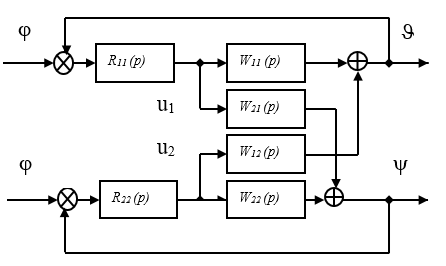
\includegraphics[width=0.8\linewidth]{img-14} 
	\caption{Структурная схема САУ}
	\label{fig:img-14}
\end{figure}

Обозначения: 
\begin{itemize}
	\item $\varphi_1, \varphi_2$ – входные координаты,
	\item $u_1, u_2$ - управляющие напряжения,
	\item $\vartheta,\psi$ - выходные координаты.
\end{itemize}
 
\textbf{1. Оценка перекрестных связей.} \label{sec:ch2/sec5/s1}
Оценим прямые и перекрестные связи САУ по их частотным характеристикам (ЧХ). 
Разомкнем один из каналов управления (рисунок~\ref{fig:img-14}) и запишем передаточную функцию (ПФ) разомкнутой системы с учетом 2-ого замкнутого канала управления при $\varphi_2=0$ (рисунок~\ref{fig:img-14}). 
В работе \cite[]{Karpov} показано, что ПФ разомкнутой системы приводится к виду (\labelcref{eq:p2:12-}), который можно упростить и оценить при слабых перекрестных связях ($\left| \delta(j\omega) \right| <<1$) 

\begin{equation}
\label{eq:p2:12-}
\begin{alignedat}{4}
W_{\textit{раз1}}\left(p\right)=
R_{11}\left(p\right)W_{11}\left(p\right)\left[1+\delta{}\left(p\right)W_2\left(p\right)\right]=\\
R_{11}\left(p\right)W_{11}\left(p\right){\Delta{}}_1\left(p\right)\cong{}\\
R_{11}\left(p\right)W_{11}\left(p\right) ,
\end{alignedat}
\end{equation}

где $W_{2}(p)=\frac{R_{22}(p)W_{22}(p)}{1+R_{22}(p)W_{22}(p)}$, 

$\delta{}(p)=\frac{W_{12}(p)W_{21}(p)}{W_{1}(p)W_{22}(p)}=\delta{}_{12}(p)\delta{}_{21}(p)$,

\begin{equation}
\label{eq:p2:14-1}
\begin{alignedat}{2}
{\Delta{}}_1(j\omega{})=[1+\delta{}(j\omega{})W_2(j\omega{})])=\left\vert{}{\Delta{}}_1(j\omega{})\right\vert{}e^{j{\phi{}}_1(\omega{})}
\end{alignedat}
\end{equation}

с оценками упрощения в частотной области по амплитудной и фазовой характеристикам: 
\begin{equation}
\label{eq:p2:13-}
\begin{alignedat}{2}
\Delta{}_1(\omega{})\ <\ 1+M_2\delta{}(\omega{})<\ 1+M_2\delta{},\\
\phi{}_1(\omega{})=arcsin(M_2\delta{}(\omega{}))<\ arcsin(M_2\delta{}\ )
\end{alignedat}
\end{equation}
где 
$\delta{}=max_{\omega{}\in{}\Omega{}}\left\vert{}\delta{}(j\omega{})\right\vert{},M_i=max_{\omega{}\in{}\Omega{}}W_i(\omega{}),(i=1,2)$ - показатели колебательности i-х каналов управления.

Если в соответствии с оценками (\labelcref{eq:p2:13-}) построить годограф
$W_{\textit{раз1}}\left(p\right)=R_{11}\left(p\right)W_{11}\left(p\right)$
и трубку вокруг него с радиусами 
${\epsilon{}}_1\left(\omega{}\right)=R_{11}\left(\omega{}\right)W_{11}\left(\omega{}\right)\delta{}\left(\omega{}\right)M_2$, 
то на основе критерия Найквиста можно судить об устойчивости системы (\labelcref{eq:p2:10-}) с учетом перекрестных связей и о влиянии перекрестных связей на ее устойчивость. Аналогичные выражения и заключения получены и для 2-го канала управления
\begin{equation}
\label{eq:p2:14-}
\begin{alignedat}{2}
W_{\textit{раз2}}\left(p\right)=R_{22}\left(p\right)W_{22}\left(p\right)\left[1+\delta{}\left(p\right)W_1\left(p\right)\right]=\\
R_{22}\left(p\right)W_{22}\left(p\right){\Delta{}}_2\left(p\right)\cong{}\\
R_{22}\left(p\right)W_{22}\left(p\right),\left(14\right)
\end{alignedat}
\end{equation}

где $W_{1}(p)=\dfrac{R_{11}(p)W_{11}(p)}{1+R_{11}(p)W_{11}(p)}$, 

$\delta{}(p)=\dfrac{W_{12}(p)W_{21}(p)}{W_{1}(p)W_{22}(p)}=\delta{}_{12}(p)\delta{}_{21}(p)$,

\begin{equation}
\label{eq:p2:15-}
\begin{alignedat}{2}
{\Delta{}}_2(j\omega{})=[1+\delta{}(j\omega{})W_1(j\omega{})])=\left\vert{}{\Delta{}}_2(j\omega{})\right\vert{}e^{j{\phi{}}_2(\omega{})}
\end{alignedat}
\end{equation}

\begin{equation}
\label{eq:p2:15-2}
\begin{alignedat}{2}
\Delta{}_2(\omega{})\ <\ 1+M_1\delta{}(\omega{})<\ 1+M_1\delta{},\\
\phi{}_2(\omega{})=arcsin(M_1\delta{}(\omega{}))<\ arcsin(M_1\delta{}\ )
\end{alignedat}
\end{equation}

\textbf{2. Оценка показателей колебательности.} \label{sec:ch2/sec5/s2}
Показатель колебательности является наиболее информативным частотным критерием оценки качества регулирования и устойчивости САУ. Пусть М1, М2 - показатели колебательности изолированных САУ (без учета перекрестных связей). С учетом сделанных выше обозначений в работе \cite[]{Karpov} получены оценки показателей колебательности каналов управления с учетом перекрестных связей

\begin{equation}
\label{eq:p2:16-}
\begin{alignedat}{2}
\overline{M_1}<M_{11}\frac{1+M_2\delta{}}{1-M_2M_1\delta{}}\\
\overline{M_2}<M_{22}\frac{1+M_1\delta{}}{1-M_1M_2\delta{}}
\end{alignedat}
\end{equation}
где 
$\delta{}={\delta{}}_{12}{\delta{}}_{21}$,
${\delta{}}_{12}=max_{\omega{}\in{}\Omega{}}{\delta{}}_{12}\left(\omega{}\right)$, 
${\delta{}}_{21}=max_{\omega{}\in{}\Omega{}}{\delta{}}_{21}\left(\omega{}\right)$,
${\delta{}}_{12}\left(\omega{}\right)=\frac{W_{12}\left(\omega{}\right)}{W_{11}\left(\omega{}\right)}$, 
${\delta{}}_{21}\left(\omega{}\right)=\frac{W_{21}\left(\omega{}\right)}{W_{22}\left(\omega{}\right)}$.

С учетом оценок (\labelcref{eq:p2:12-,eq:p2:16-}) сформулируем условия декомпозируемости для двухканальных систем.

\textbf{Определение.}
 Если i-е изолированные каналы разомкнутых систем управления устойчивы и выполняются условия: 
\begin{enumerate}
	\item $\omega \in [0,\inf)$,
	\item $\delta{}_{12}\left(\omega{}\right)<1$, 
	$\delta{}_{21}\left(\omega{}\right)<1$
	${\delta{}}_i(\omega{})={\delta{}}_{12}(\omega{}){\delta{}}_{21}(\omega{})M_j<\delta^{\textit{доп}}(M^{\textit{доп}}, \varDelta^{\textit{доп}}, \varphi^{\textit{доп}}) (i=1,2; j=2,1)$
	\item годографы 
	$W_{\textit{разi}}(j\omega{})=W_{ii}(j\omega{})W_{ii}(j\omega{})$ с трубкой радиуса 
	${\epsilon{}}_1\left(\omega{}\right)$ не охватывают точку $(-1,j0)$,
	\item оценки показателей колебательности $\overline{M_1}<M^{\textit{доп}}$,
\end{enumerate}
то декомпозиция системы (\labelcref{eq:p2:11-}) приемлема в смысле устойчивости и качества регулирования САУ; где
$\delta^{\textit{доп}}(M^{\textit{доп}}, \varDelta^{\textit{доп}}, \varphi^{\textit{доп}})$
 – функциональная зависимость точности декомпозируемости каналов управления от допустимых требований качества регулирования $M^{\textit{доп}}$ и запасов устойчивости $\varDelta^{\textit{доп}}, \varphi^{\textit{доп}}$ САУ. 
 
 
 Методика оценки перекрестных связей:
 
 1.
 
 2.
 
 
\section{Синтез регуляторов частотным методом} \label{sec:ch2/sec6}


Синтез регуляторов проводится с учетом управляющих воздействий (\labelcref{eq:p2:3-a2}) и действующих моментов в классе комбинированных астатических систем, исходя из условий устойчивости, точности и качества регулирования. 
\begin{equation}
\label{eq:p2:3-a2}
\begin{alignedat}{2}
\alpha_1(t) = A_1\sin(\omega_1t) ,\\
\alpha_2(t) = A_2\sin(\omega_2t) ,\\
\alpha_3(t) = bt \neq 0,\\
\alpha_{\textit{В}}(t) = A_4\sin(\omega_4t) ,\\
\end{alignedat}
\end{equation}
где $\alpha_{\textit{В}}(t)$ - смещения изображения от действия вибраций,
$\alpha_1(t), \alpha_2(t)$ - расфокусировки и динамических погрешностей систем сканирования и слежения,
$\alpha_3(t)$ - движение объекта наблюдения (ОН), 
$A_i$ - амплитуда соответствующих гармонических колебаний,
$\omega_i$ - частота соответствующих гармонических колебаний,
$b$ - скорость движения объекта наблюдения.

Предварительно выбираются привода с учетом моментов нагрузки ($M_{\textit{н}}$), скоростей и ускорений и носителя \cite[]{Babaev38-a2-13}. Модуль частотной характеристики разомкнутых изолированных каналов управления синтезируется из условия 

\begin{equation}
\label{eq:p2:14-a2}
\begin{alignedat}{2}
\left| W (j\omega) \right| \geqslant \dfrac{\varepsilon_1 A_1 + \varepsilon_2 A_2 + b + A_2 + k_f M_i }{\varDelta\alpha} ,
\varDelta\alpha = \varDelta\alpha^{\textit{доп}}_{\textit{Л}} + \varDelta\alpha^{\textit{доп}}_{\textit{Г}} + \varDelta\alpha^{\textit{доп}}_{\textit{В}}
\end{alignedat}
\end{equation}

где $\epsilon_i \leq (0.03-0.1)$ – точности инвариантности к колебаниям носителя, $k_f$ – коэффициент передачи привода по моменту. Постоянные времени привода ($T_{\textit{П}}$), усилителя ($T_{\textit{У}}$), датчика ($T_{\textit{д}}$) определяется из условий устойчивости 
(при $T_{\textit{П}}>T_{\textit{У}}>T_{\textit{д}}$) 
и показателя колебательности (М) \cite[]{Bessekerski-a2-14}:	

\begin{equation}
\label{eq:p2:15-a2}
\begin{alignedat}{2}
k_v \leq \dfrac{T_{\textit{Д}}+T_{\textit{У}}+T_{\textit{П}}}{T_{\textit{П}}(T_{\textit{У}}+T_{\textit{Д}})} ,\\
T_{\textit{П}} = \dfrac{M^2 + M\sqrt{M^2-1}}{2k_v} ,\\
T_{\textit{Д}} \leq \dfrac{1}{10k_v} ,\\
T_{\textit{У}} \leq \dfrac{1}{40k_v}\\
\end{alignedat}
\end{equation}

Если условия (\labelcref{eq:p2:15-a2}) не выполняются, то далее синтез проводится путем построения желаемых логарифмических амплитудных и фазовых характеристик (ЛАХ-$L(\omega)$, ЛФХ-$\varphi(\omega)$), реализующих требования устойчивости (критерий Найквиста) и качества регулирования (частотные свойства разомкнутой системы) \cite[]{Bessekerski-a2-14}:

\begin{itemize}
	\item в низкочастотной области ЛАХ – $20 lg(\alpha_{\textit{вх}}(\omega_{\textit{н}}) / \varDelta\alpha)=L(\omega_{\textit{н}})<L(\omega)$, 
	$20 lg K_c < L(\omega)$, где 
	$\omega_{\textit{н}}$ – частоты колебаний носителя;
	\item в среднечастотной области ЛАХ – на частоте среза ($\omega_{\textit{ср}}$) наклон ЛАХ должен быть -20 дб/дек в диапазоне частот: \\
	$\varDelta\omega = \omega_c ( 1 \pm 0.5(M + 1)/(M - 1) )$, где М – показатель колебательности;
	\item запасы устойчивости – 
	по фазе $\varDelta\varphi>45-60$ град. и 
	по амплитуде $\varDelta L>6$ дБ,
	которые определяют указанные требования к параметрам датчиков, усилителей и корректирующих звеньев, последние определяются по формулам:
	\begin{equation}
	\label{eq:p2:16-a2}
	\begin{alignedat}{2}
	W_{\textit{кз}}(p) = \dfrac{T_2p+1}{T_3p+1} ,\\
	T_2 \geq \dfrac{M}{\omega_{\textit{ср}}(M-1)} ,\\
	T_3 \leq \dfrac{M}{\omega_{\textit{ср}}(M+1)}
	\end{alignedat}
	\end{equation}
\end{itemize}

Далее синтез доопределяется на основе исследования динамики САУ на пространственной компьютерной модели \cite[]{Malivanov-a2-9} с учетом нелинейностей регулятора и объекта управления.

\section{Разработка компьютерной имитационной модели} \label{sec:ch2/sec7}

Методика построения КИМ:

1.

2.


\section{Разработка макета, исследование и испытания } \label{sec:ch2/sec8}

\textbf{Разработка и исследование масштабного динамического макета}

Необходимость создания и исследования динамического макета (ДМ) возникает при разработке принципиально новых и модернизируемых САУ БОЭП с целью проверки заложенных принципов управления и стабилиза-ции изображения,что позволяет сократить стоимость и время их разработки. 

Размеры (L) и массы (m) ОУ (его узлов и деталей), необходимых мощностей (Р) и моментов (М) приводов, сил пружин амортизаторов (F) ДМ определяются, исходя из выбранных масштабов ($\mu_i$) динамического подобия \cite[]{Babatko-a2-17}:

\begin{equation}
\label{eq:p2:23-a2}
\begin{alignedat}{2}
\mu_i=a_m / a, (i=L, \rho, m, P, M, F); \mu_t=\mu_x=\mu_\varphi=1 ,
\end{alignedat}
\end{equation}
где 
$a_m$ – параметр ДМ, 
$a$ – натуральный параметр прибора, 
$\rho$ - плотности материалов, 
$t$ – текущее время, 
$x, \varphi$ - линейные и угловые движения ОУ.

Далее разработка, создание и исследование динамики ДМ проводится в следующей последовательности:
\begin{itemize}
	\item определяются параметры ДМ, его приводов и СА с учетом (\labelcref{eq:p2:23-a2}); 
	\item по рабочим чертежам БОЭП в среде SolidWorks разрабатывается сборочный чертеж ДМ и определяется его геометрия масс; 
	\item с использованием технологии 3D печати изготавливается механическая часть ДМ совместно с приводами и амортизаторами по чертежам ДМ, электронная часть САУ (датчики, усилители, корректирующие устройства) допускается в макетном исполнении; 
	\item по частотным характеристикам ДМ в соответствии с критерием (\labelcref{eq:p2:2}) синтезируются параметры САУ (\labelcref{eq:p2:14-a2,eq:p2:15-a2,eq:p2:16-a2}) и СВ и проводится 
	настройка и исследовании динамики САУ и СВ динамического макета;
	
\end{itemize}

По результатам разработки и исследований делается выбор приемлемо-сти исследуемых вариантов ДМ для дальнейшего применения.

\textbf{Испытание опытного образца на стендах}
 в соответствии с методиками испытаний и требований ТЗ. Если критерии (\labelcref{eq:p2:2}) не выполняются, то проводится анализ результатов и возврат к доопределению модели или ТЗ. Результаты испытаний отражают в протоколе и делают заключение о необходимости доработок СВ и САУ и проведения повторных испытаний или допуске их к испытаниям на борту. 

\begin{comment}
\textbf{Испытания на борту}
 в соответствии с методиками натурных испытаний и требований ТЗ. Если критерии (\labelcref{eq:p2:2}) не выполняются, то переходим на проводится анализ результатов и возврат к доопределению модели или ТЗ. Результаты испытаний и требования к техническим характеристикам СВ и САУ фиксируем в протоколе испытаний и делаем заключение о необходимости доработок СВ и САУ или допуске их к дальнейшему производству.
\end{comment}
\begin{comment}
Приведенная методика была апробирована при разработке ряда САУ ОЭП \cite[]{Belyakov}, \cite[]{Torshina},\cite[]{Malivanov-a2-9}, \cite[]{Burdinov-a2-10}, \cite[]{Sokolski22}, \cite[]{Dubovik-a2-12}. Каждому из блоков на рисунке~\ref{fig:tikz_example} присущи своя специфика и его математическое или логическое описание и предполагается соответствующая методика его реализации. Сущность их раскроем ниже.
\end{comment}

\section{Выводы по главе} \label{sec:ch2/sec9}

1. Разработана интерактивная итерационная методика разработки и испытания бортовых ОЭП. Предлагаемая методика разработки и исследования, объединяя теорию оптического изображения, теорию автоматического управления и законы механики, методы математического и компьютерного моделирования и испытаний в единое целое, позволяет решать важные прикладные задачи построения адекватных математических моделей бортовых ОЭП как объектов управления. На их основе с применением компьютерных технологий наиболее эффективно можно решать задачи синтеза САУ бортовых ОЭП, что позволит уменьшить сроки и стоимость их разработки

2. Предложена методика оценки допусков на точность стабилизации изображения БОЭП, находящихся в сложных механических и температурных воздействиях

3.  Представленная методика построения имитационной модели компьютерной в пакете учитывает специфику управления ОЭП и нелинейности и нестационарности объекта управления 

4. Предложенная методика оценки перекрестных связей позволяет проводить декомпозицию двухсвязной системы с применением компьютерных технологий.

\clearpage